\documentclass{article}

\usepackage[a4paper]{geometry}
\usepackage[spanish]{babel}
\usepackage{xcolor}
\usepackage{placeins}

\usepackage{mathbbol}
\usepackage{amsmath}
\usepackage{amsfonts}
\usepackage{hyperref}
\usepackage{graphicx}
\usepackage{subcaption}

\usepackage{algorithm}
\usepackage{algpseudocode}

% Cambiar 'Cuadro' -> 'Tabla'
\addto\captionsspanish{
    \renewcommand{\tablename}{Tabla}
}

\begin{document}

\begin{center}
    {\Large Aprendizaje Automático para Datos en Grafos} \\
    {\LARGE \textbf{Laboratorio 4}} \\
    \vspace{2em}
    \begin{minipage}{0.45\textwidth}
        \centering
        Graciana Castro \\
        4.808.848-2 \\
        gcastro@fing.edu.uy
    \end{minipage}
    \hfill
    \begin{minipage}{0.45\textwidth}
        \centering
        Julian O'Flaherty \\
        6.285.986-9 \\
        julian.o.flaherty@fing.edu.uy
    \end{minipage}
\end{center}


\section{Introducción}

\section{Inferencia de topología en datos sintéticos}

\subsection{Generación del grafo sintético}

Para generar un grafo sintético, utilizaremos el siguiente algoritmos:
\begin{enumerate}
    \item Sorteamos $N$ puntos de forma uniforme en el cuadrado $[0,1] \times [0,1]$. Esos serán los vértices de nuestro grafo.
    \item Para cada par de puntos $i$ y $j$ que sorteamos antes, tomamos como peso de la arista
    \begin{equation*}
        w_{ij} = \begin{cases}
            0 & \text{si } i=j \\
            e^{-\frac{d(i,j)}{2\sigma^2}} & \text{si } i \neq j
        \end{cases}
    \end{equation*}
    donde $d(i,j)$ es la distancia euclidea en $\mathbb{R}^2$ y $\sigma$ es un parámetro fijo.
    \item Descartamos las aristas cuyo peso $w_{ij}$ sea menor que un número fijo $r>0$.
\end{enumerate}
En la figura~\ref{fig:grafo_sintetico} se muestra un grafo sintético generado con el algoritmo anterior para $N=50$, $\sigma=0.5$ y $r=0.6$.

\begin{figure}[htb]
    \centering
    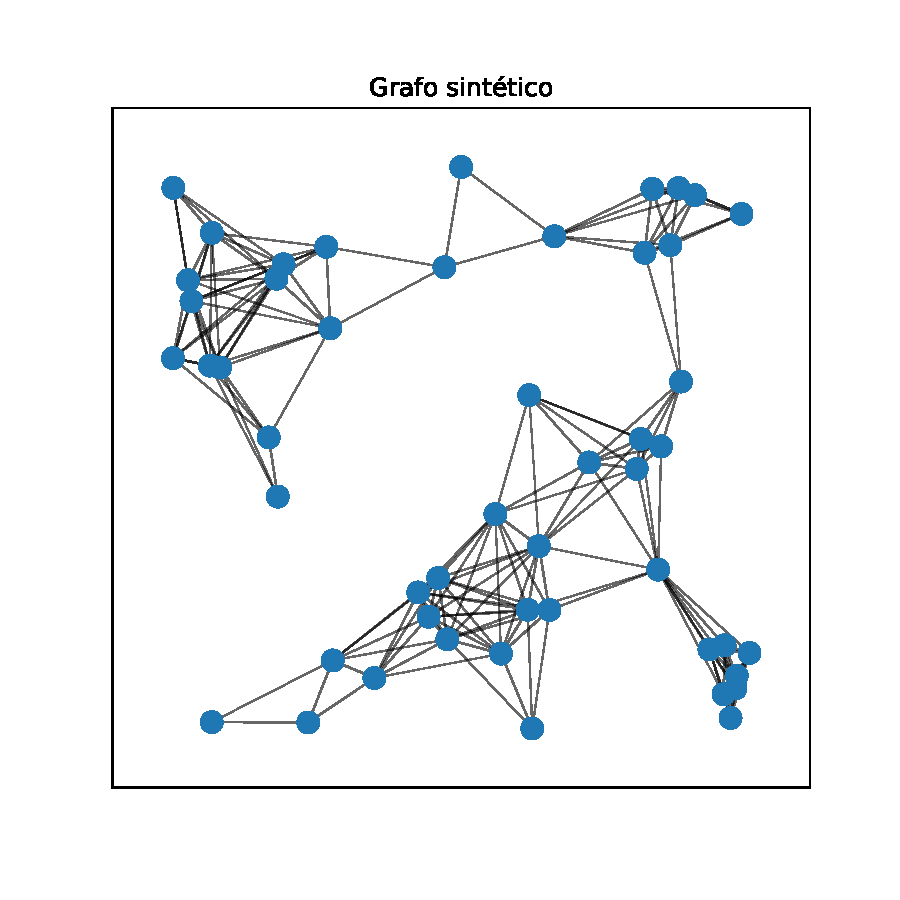
\includegraphics[width=0.5\textwidth]{imagenes/grafo_sintetico.pdf}
    \caption{Grafo sintético generado con $N=50$, $\sigma=0.5$ y $r=0.6$.}
    \label{fig:grafo_sintetico}
\end{figure}

A cada nodo del grafo sintetico, le asignaremos una señal $x_i \sim \mathcal{N}(0, \mathbf{L}^\dagger)$, donde $\mathbf{L}^\dagger$ es la pseudoinversa de la matriz laplaciana $\mathbf{L}$ del grafo. En la figura~\ref{fig:signals_X_pseudoinverse} se muestra un sample de señales
donde cada columna $j$ es la señal asociada al nodo $j$ del grafo. La cantidad de filas, o el tamaño de la muestra, es el parámetro $n_{\text{samples}}$ del algoritmo, por lo que si $n_samples$ es menor que $N$, la matriz de covarianza empírica no es invertible.

\begin{figure}[htb]
    \centering
    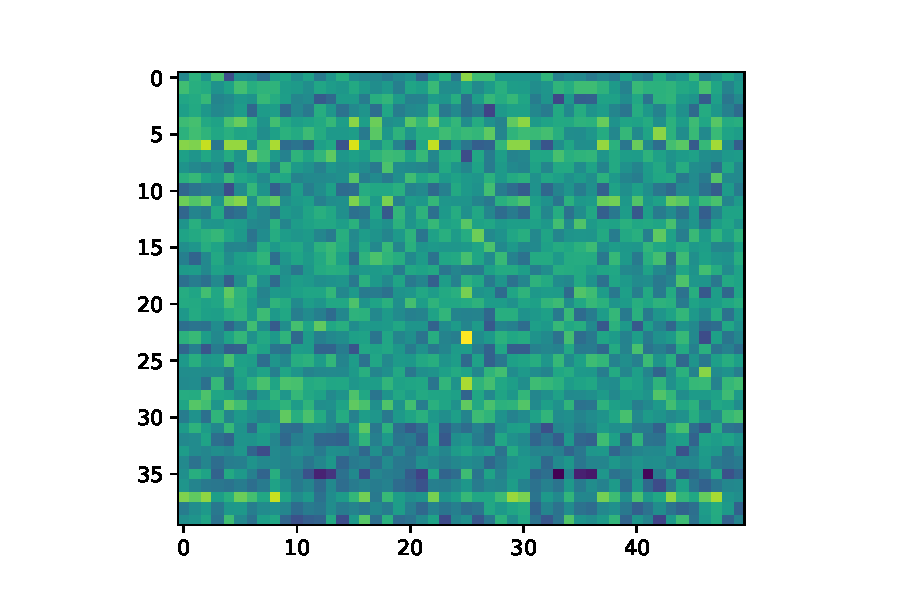
\includegraphics[width=0.6\textwidth]{imagenes/signals_X_pseudoinverse.pdf}
    \caption{Sample de señales asignadas a los nodos del grafo sintético.}
    \label{fig:signals_X_pseudoinverse}
\end{figure}

\subsection{Estimación de estructura con Graphical Lasso}

Estimaremos la estructura del grafo a partir de la matriz de datos utilizando el Graphical Lasso. Este método busca al estimador 
de máxima verosimilitud de la matriz de precisión $\boldsymbol{\Theta}$ que cumple:
\begin{equation}
\hat{\boldsymbol{\Theta}} = \arg \max_{\boldsymbol{\Theta} \succeq 0} \left\{ \log \det \boldsymbol{\Theta} - \text{trace}(\hat{\boldsymbol{\Sigma}} \boldsymbol{\Theta}) - \lambda \|\boldsymbol{\Theta}\|_1 \right\}
\end{equation}
Una de las propiedades importantes del Graphical Lasso, es que cuando $\lambda =  2\sqrt{\frac{\log N}{P}}$,
\begin{equation*}
    \|\hat{\boldsymbol{\Theta}} - \boldsymbol{\Theta}_0\|_2 \leq \sqrt{\frac{d_{\max}^2 \log N}{P}} \quad \text{w.h.p.}
\end{equation*}

\begin{figure}[htb]
    \centering
    \begin{subfigure}[t]{0.32\linewidth}
        \centering
        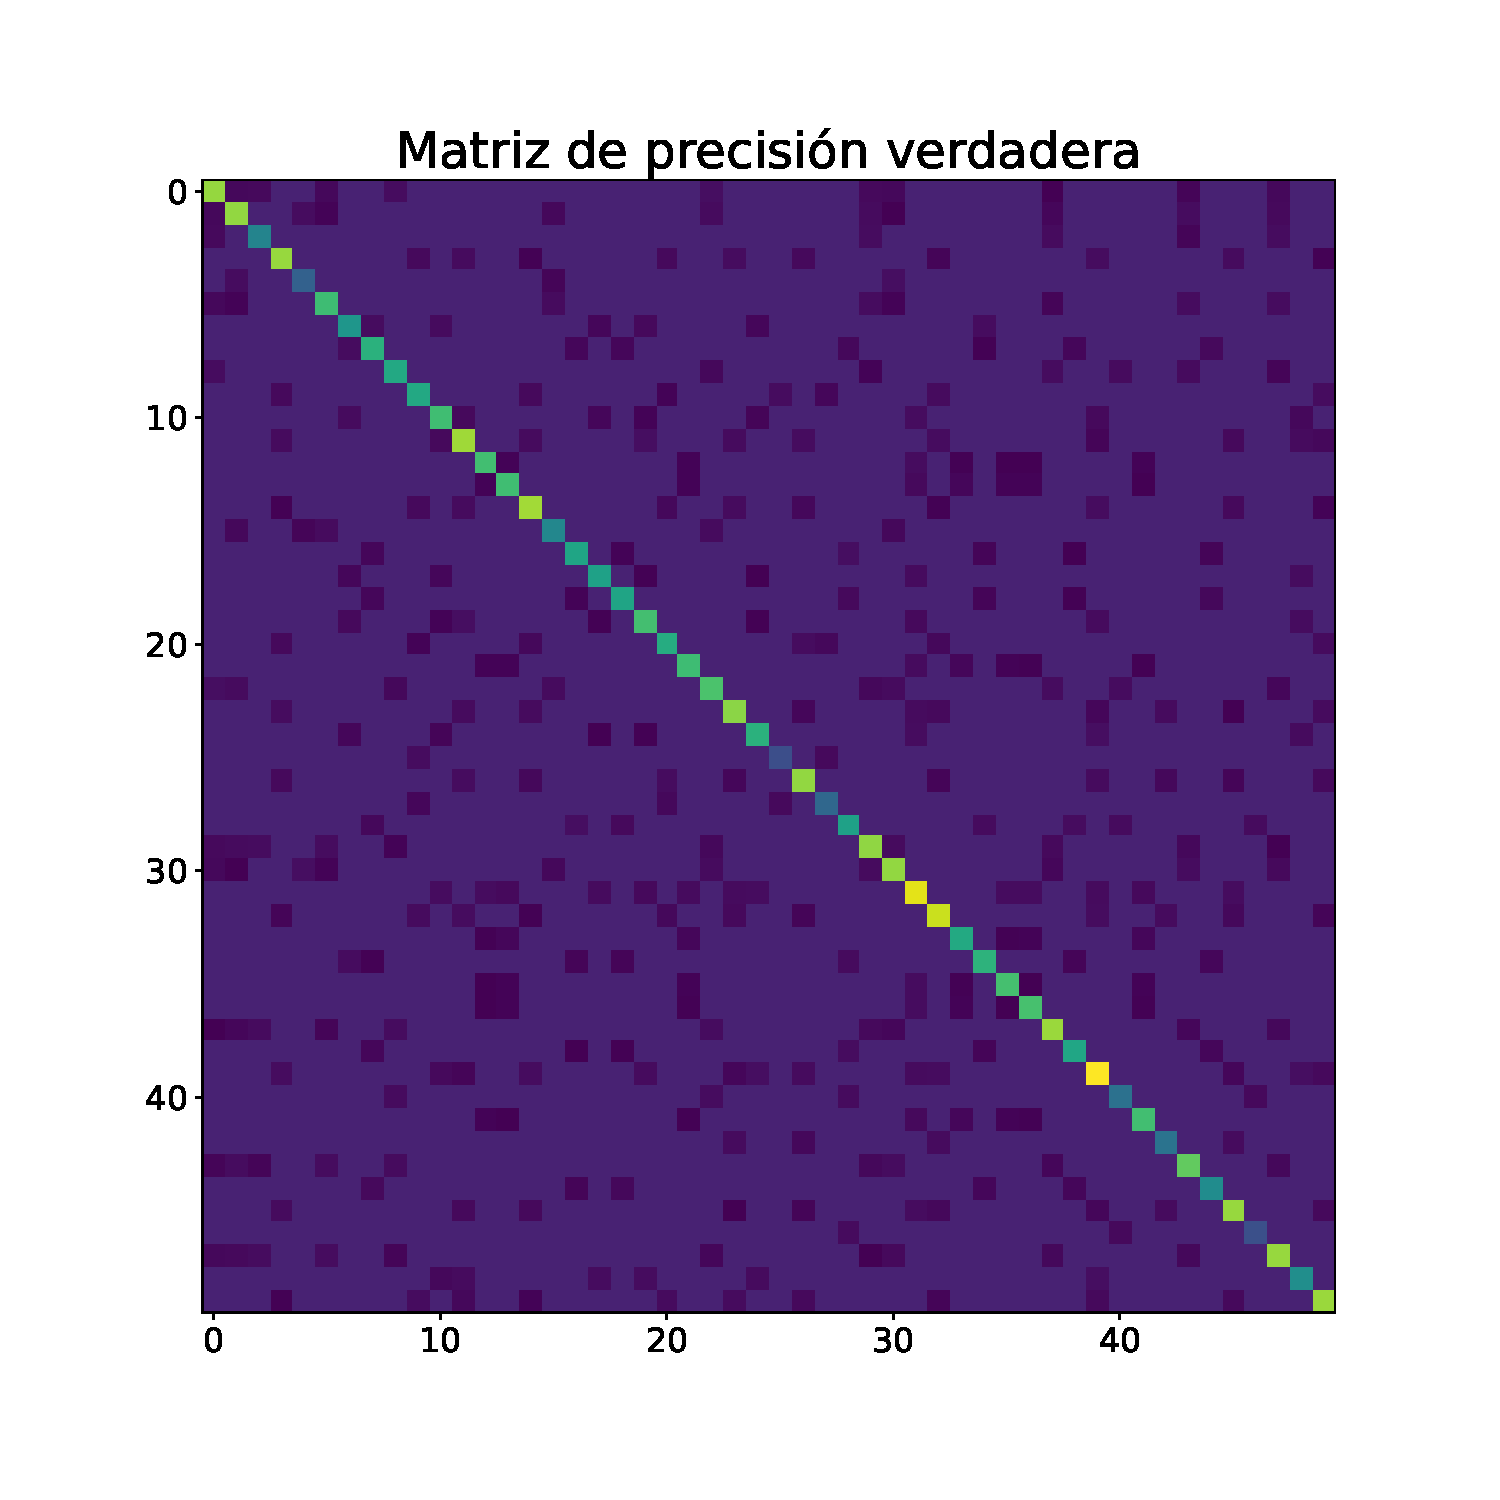
\includegraphics[width=\textwidth]{imagenes/graphical_lasso/true_precision_sample.pdf}
        \caption{Precisión verdadera}
        \label{fig:graphical_lasso_true_precision}
    \end{subfigure}\hfill
    \begin{subfigure}[t]{0.32\linewidth}
        \centering
        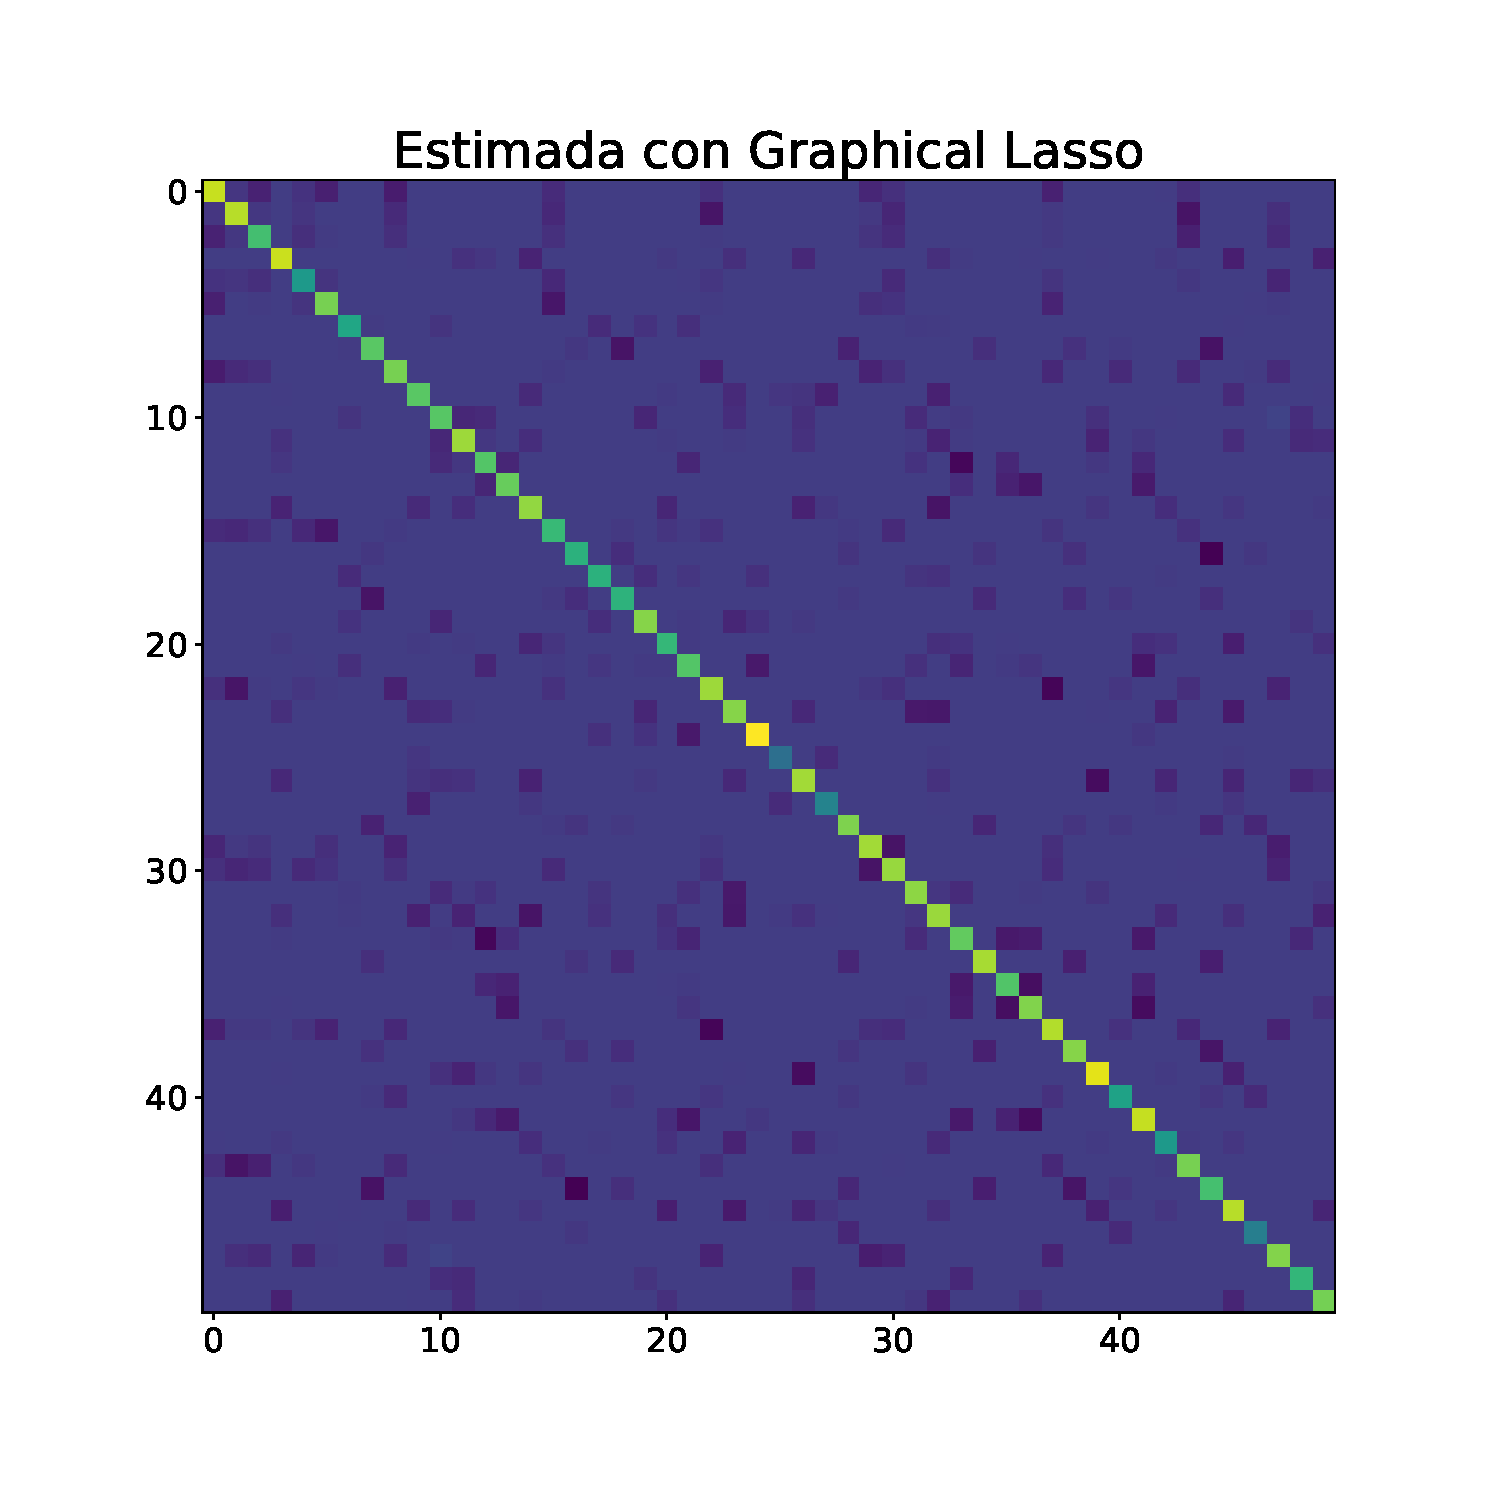
\includegraphics[width=\textwidth]{imagenes/graphical_lasso/graphical_sample.pdf}
        \caption{Estimación mediante Graphical Lasso}
    \end{subfigure}\hfill
    \begin{subfigure}[t]{0.32\linewidth}
        \centering
        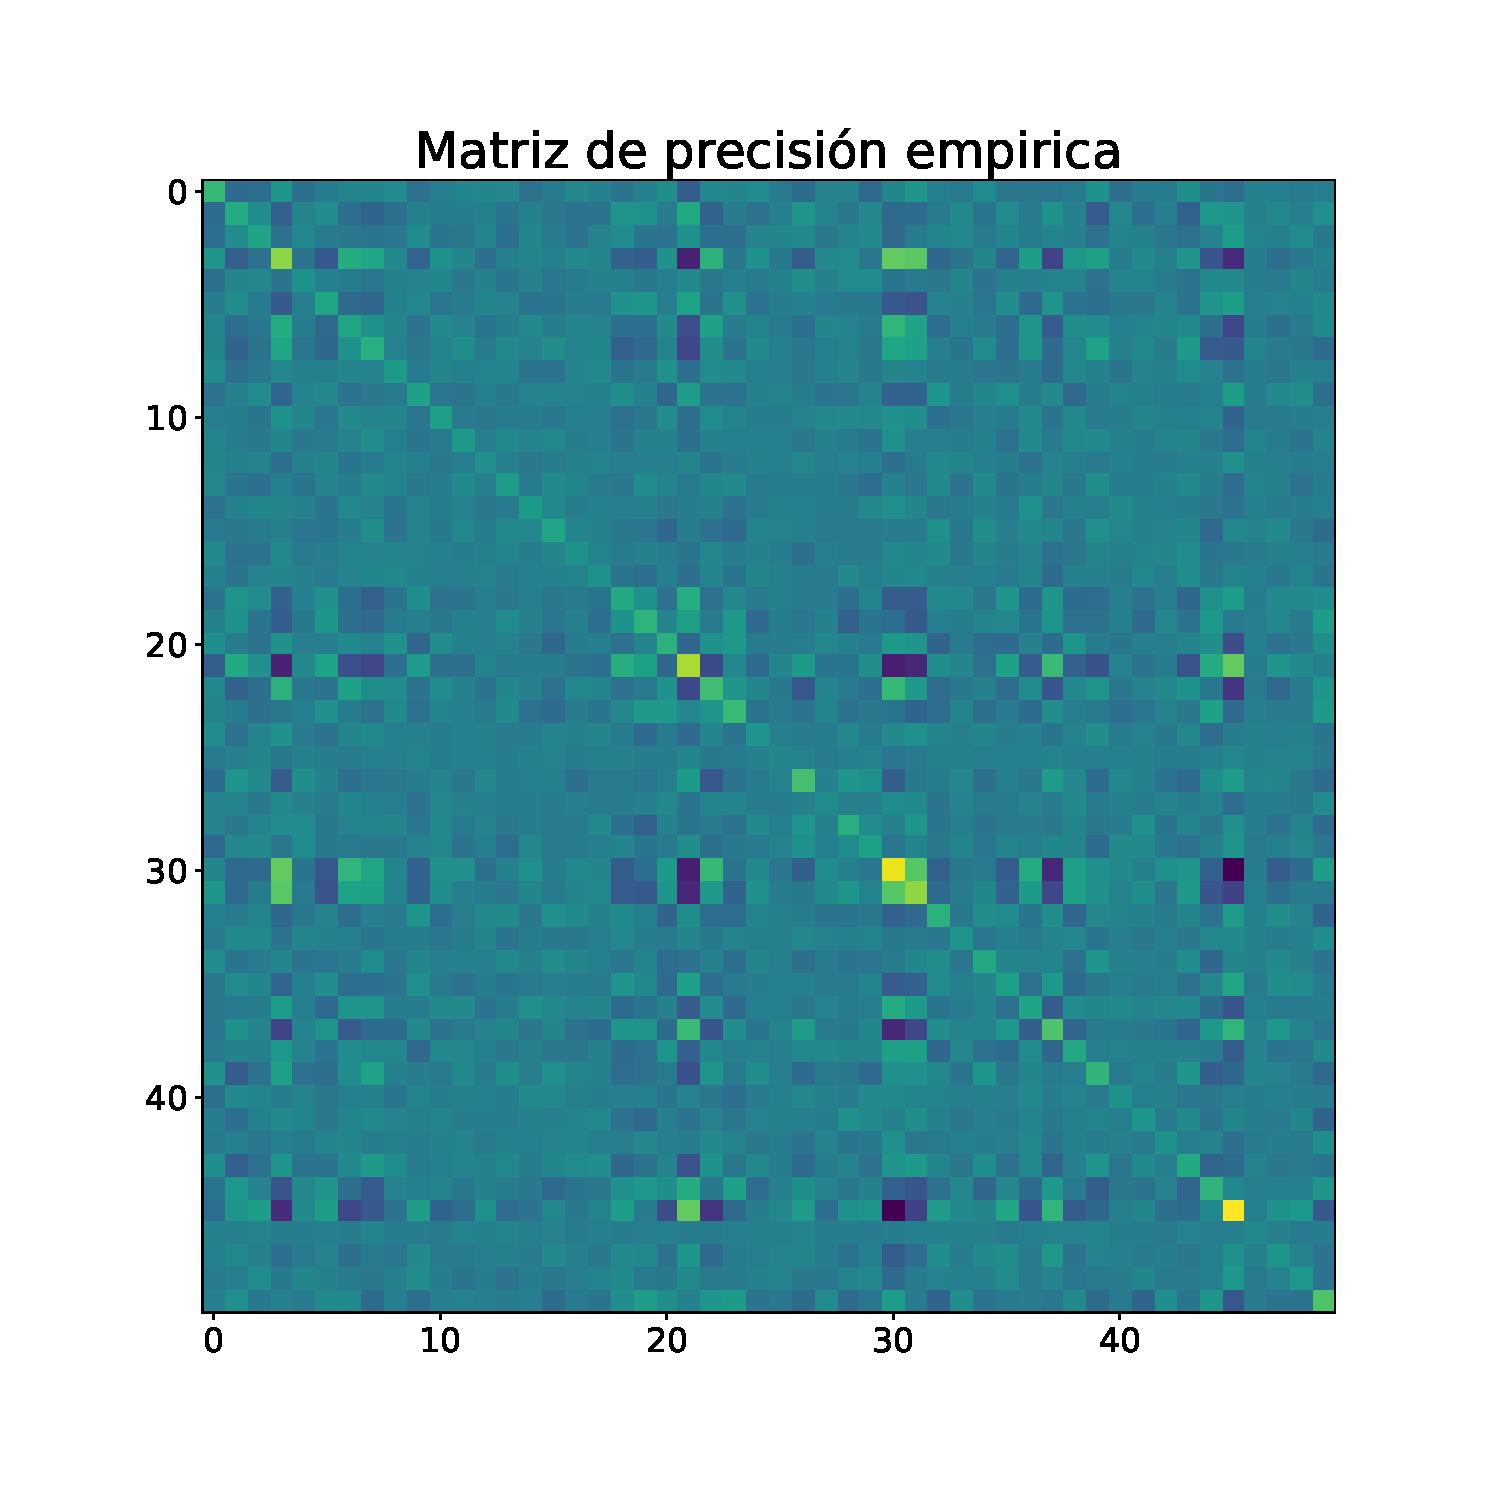
\includegraphics[width=\textwidth]{imagenes/graphical_lasso/estimated_sample.pdf}
        \caption{Estimación Graphical Lasso}
    \end{subfigure}
    \caption{Comparación entre la matriz de precisión verdadera, la estimación mediante Graphical Lasso y la estimación obtenida con empíricamente ($\Theta = \Sigma^{-1}$), cuando $n_{\text{samples}}=40$ y $N=50$}
    \label{fig:graphical_lasso_triptych}
\end{figure}
En la figura~\ref{fig:graphical_lasso_triptych} se puede observar la estimación obtenida con \emph{Graphical Lasso} comparada con la estimación empírica cuando el número de samples utilizado $n_{\text{samples}}$ es menor que la cantidad de nodos $N$. En este caso, la estimación
empírica resulta mala, dado que la matriz de covarianza empírica no es invertible. El método de \emph{Graphical Lasso} obtiene un resultado muy similar a la matriz de precisión verdadera, donde el valor de $\lambda$ se calcula mediante cross validation. 

En la figura~\ref{fig:graphical_lasso_alpha_comparison} observamos el efecto del variar el valor de lambda sobre la matriz de precisión estimada. A medida que aumenta la regularización, la matriz va perdiendo zeros tendiendo a una matriz diagonal, lo cual es esperable
dado que el valor de lambda esta asociado a la norma 1 de la matriz de precisión. 
\begin{figure}[htb]
    \centering
    \begin{subfigure}[t]{0.32\linewidth}
        \centering
        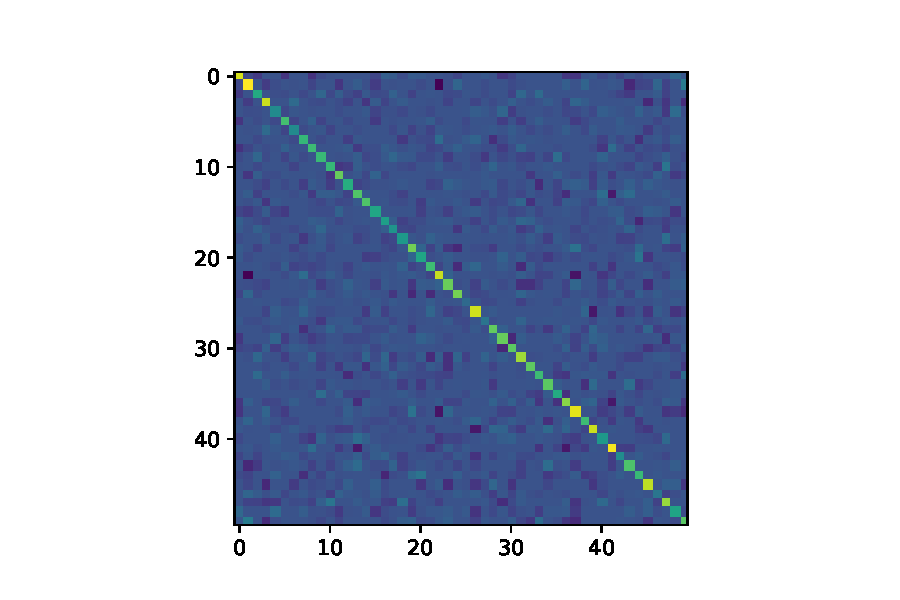
\includegraphics[width=\textwidth]{imagenes/graphical_lasso/graphical_lasso_alpha_0_01.pdf}
        \caption{$\lambda = 0.01$}
    \end{subfigure}\hfill
    \begin{subfigure}[t]{0.32\linewidth}
        \centering
        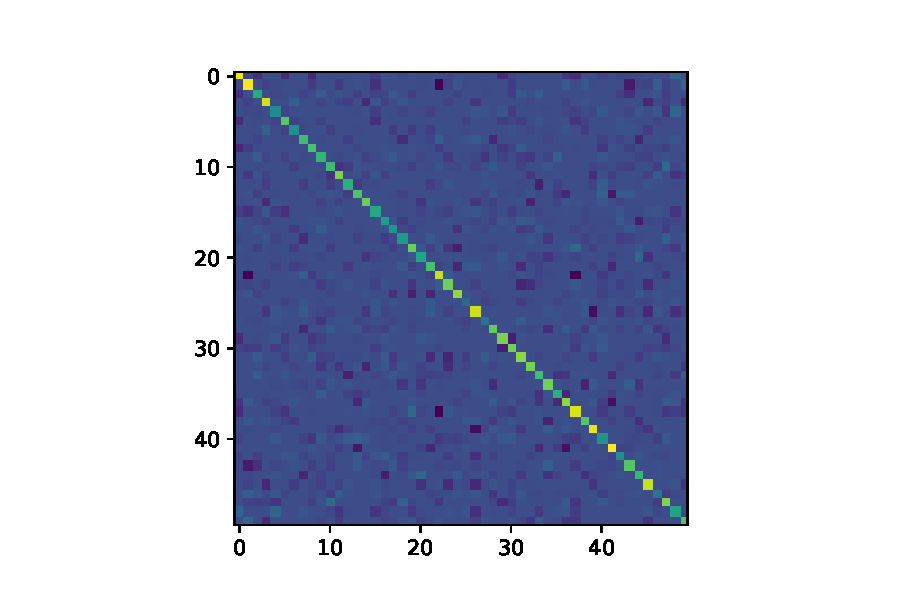
\includegraphics[width=\textwidth]{imagenes/graphical_lasso/graphical_lasso_alpha_0_02.pdf}
        \caption{$\lambda = 0.02$}
    \end{subfigure}\hfill
    \begin{subfigure}[t]{0.32\linewidth}
        \centering
        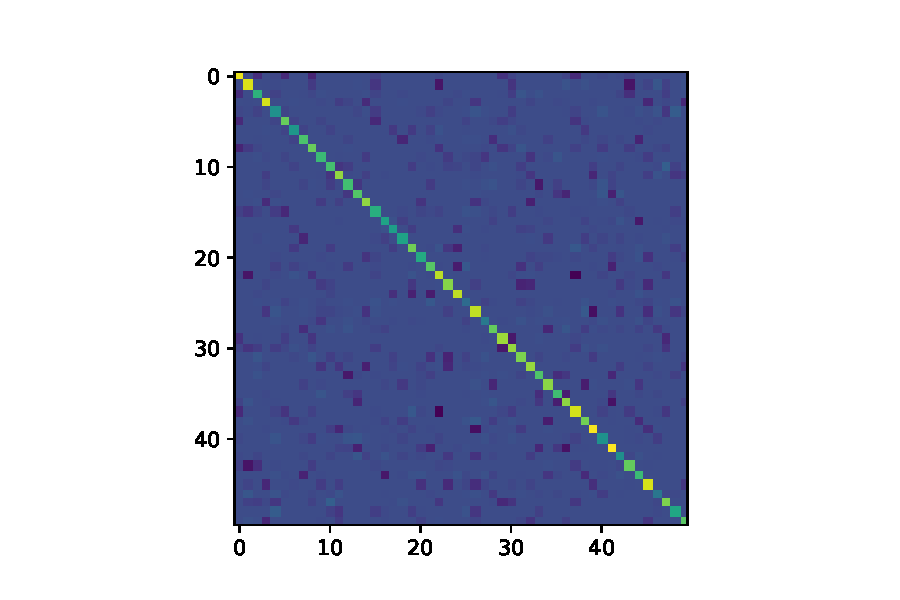
\includegraphics[width=\textwidth]{imagenes/graphical_lasso/graphical_lasso_alpha_0_05.pdf}
        \caption{$\lambda = 0.05$}
    \end{subfigure}
    \begin{subfigure}[t]{0.32\linewidth}
        \centering
        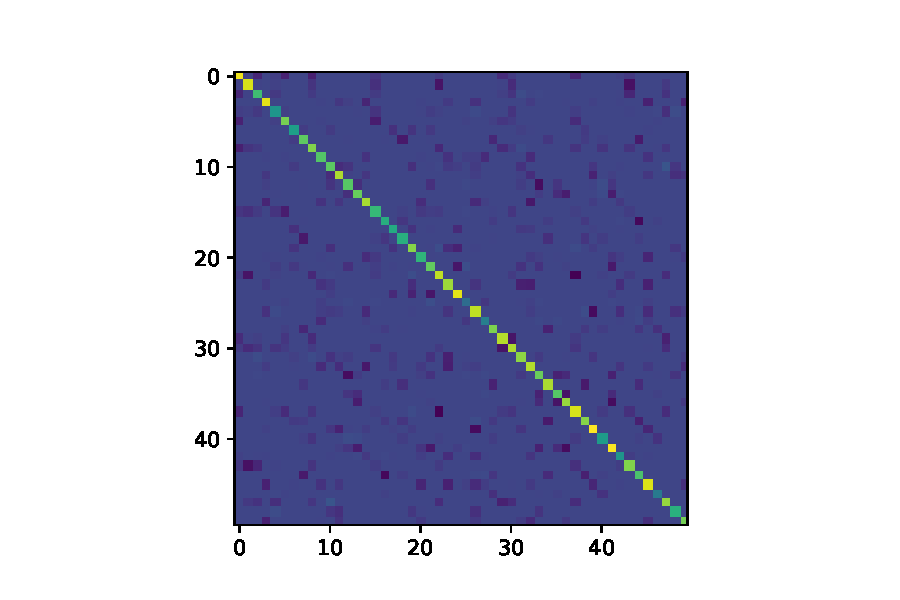
\includegraphics[width=\textwidth]{imagenes/graphical_lasso/graphical_lasso_alpha_0_1.pdf}
        \caption{$\lambda = 0.1$}
    \end{subfigure}
    \begin{subfigure}[t]{0.32\linewidth}
        \centering
        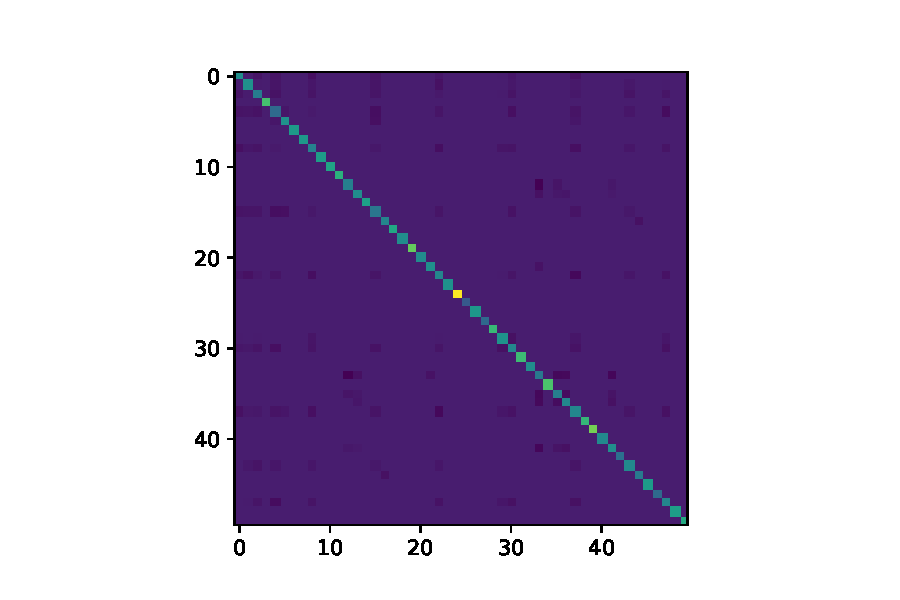
\includegraphics[width=\textwidth]{imagenes/graphical_lasso/graphical_lasso_alpha_0_5.pdf}
        \caption{$\lambda = 0.5$}
    \end{subfigure}
    \begin{subfigure}[t]{0.32\linewidth}
        \centering
        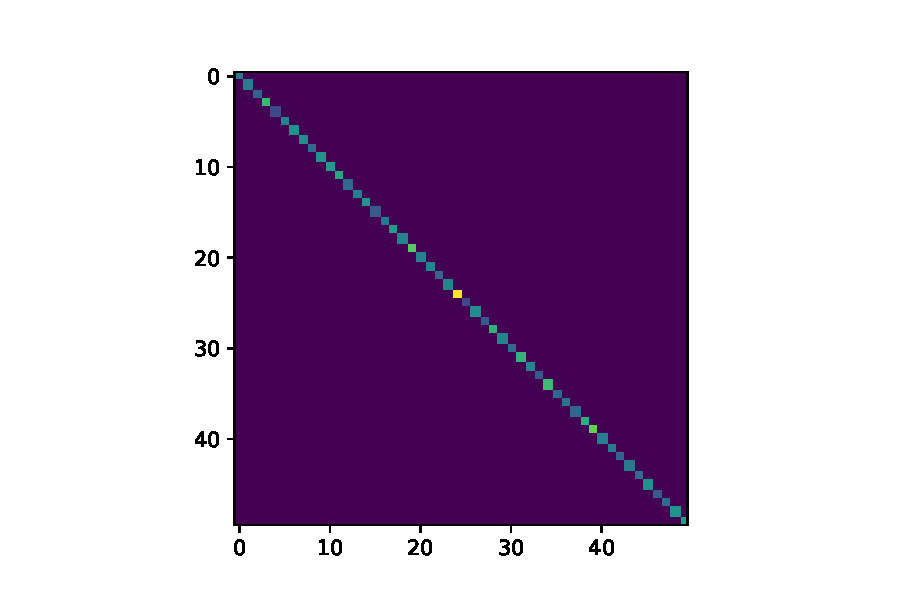
\includegraphics[width=\textwidth]{imagenes/graphical_lasso/graphical_lasso_alpha_1.pdf}
        \caption{$\lambda = 1$}
    \end{subfigure}
    \caption{Estimación mediante Graphical Lasso para distintos valores de $\lambda$. La matriz de precisión verdadera se muestra en la figura~\ref{fig:graphical_lasso_true_precision}. No se muestran valores menores a $0.01$ porque hay poca diferencia notable, y a partir de $0.005$ el sistema queda mal condicionado y no puede ser resuelto.
}
    \label{fig:graphical_lasso_alpha_comparison}
\end{figure}

\subsection{Estimación de estructura con Meinshausen y Bühlmann}



\subsection{Estimación de estructura con Kalofolias}


\subsection{Comparación y visualización de los grafos aprendidos}

\begin{figure}[htb]
    \centering
    \begin{subfigure}[t]{0.24\linewidth}
        \centering
        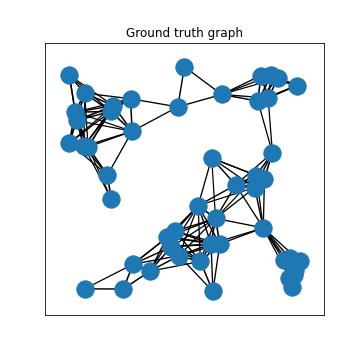
\includegraphics[width=\textwidth]{imagenes/generated_graph_syntetic/ground_truth_graph.png}
        \caption{Grafo verdadero}
    \end{subfigure}\hfill
    \begin{subfigure}[t]{0.24\linewidth}
        \centering
        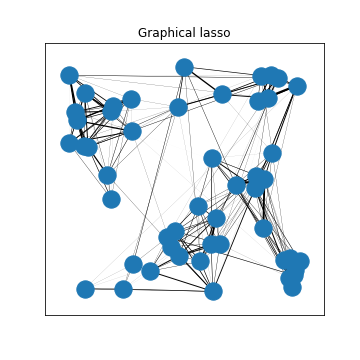
\includegraphics[width=\textwidth]{imagenes/generated_graph_syntetic/graphical_lasso.png}
        \caption{Graphical Lasso}
    \end{subfigure}\hfill
    \begin{subfigure}[t]{0.24\linewidth}
        \centering
        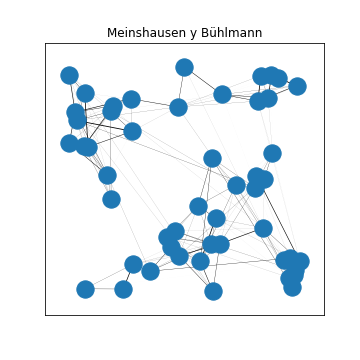
\includegraphics[width=\textwidth]{imagenes/generated_graph_syntetic/meinshausen_buhlmann.png}
        \caption{Meinshausen y Bühlmann}
    \end{subfigure}\hfill
    \begin{subfigure}[t]{0.24\linewidth}
        \centering
        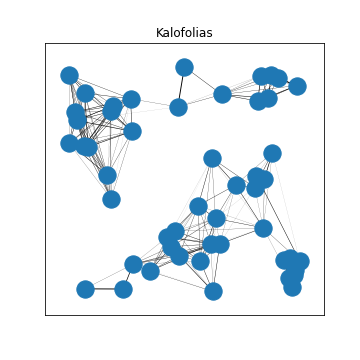
\includegraphics[width=\textwidth]{imagenes/generated_graph_syntetic/kalofolias.png}
        \caption{Kalofolias}
    \end{subfigure}
    \caption{Comparación visual de los grafos: verdadero y aprendidos por distintos métodos.}
    \label{fig:generated_graphs_syntetic}
\end{figure}

\subsection{Discusión}


\section{Inferencia de topología en MNIST}

\subsection{Descripción del dataset y preprocesamiento}

\subsection{Construcción de la matriz de features y t-SNE}

\subsection{Grafo aprendido con Meinshausen y Bühlmann}

\subsection{Grafo aprendido con Kalofolias y umbralización}

\subsection{Clustering espectral sobre grafos aprendidos}

\subsubsection{Métricas de evaluación}

\subsubsection{Resultados y comparación}

\subsection{Visualización en el plano t-SNE por método}

\subsection{Análisis de aciertos y errores por método}


\section{Conclusiones}


\section{Referencias}
\bibliographystyle{plain}
\bibliography{refs}


\end{document}